% \chapter{Methoden und Praktiken}

%\textit{In diesem Kapitel soll beschrieben werden, wie eine Nachvollziehbarkeit in Webanwendungen erreicht werden kann. Spezielle Methoden und Praktiken sollen vorgestellt und beleuchtet werden.}
% \textit{Hier könnte unter anderem \textbf{OpenTelemetry} betrachtet werden.}

\vspace{-\baselineskip}

\section{Methoden}

\subsection{Logging}

%\textit{Folgende Fragen sollen zur Methode beantwortet werden}
%\begin{enumerate}
%	\item \textit{Gibt es Besonderheiten zu Logging in anderen Projekten (Backend vs. Frontend)?}
%	\item \textit{Wie können Logs an einen auswertenden Stakeholder gelangen?}
%	\item \textit{Welches Verhalten kann hiermit aufgedeckt/nachvollziehbar gemacht werden?}
%\end{enumerate}

Mit Logging bezeichnet man die systematische Protokollierung von Softwareprozessen und ihren internen Zuständen. Mithilfe von Logs, also Protokollen, kann Betreibern und Entwicklern ermöglicht werden, dass sie das Anwendungsverhalten nachvollziehen können. Beispielsweise ist es sinnvoll einen fehlgeschlagenen Login eines Nutzers zu loggen, dabei ist es hilfreich, wenn viele Kontextinformationen mitgeloggt werden. % Nah verwandt mit oder basierend auf Logging sind die Teilgebiete Auditing, Monitoring, Tracing und Operations-Monitoring.

Logging bei Webfrontends stellt eine besondere Hürde dar, denn wie bereits in \autoref{sec:logdaten} geschildert, müssen die Logs an ein Partnersystem weitergeleitet werden.

\subsubsection{Structured Logging}

%\subsection{Monitoring}
%
%\textit{Folgende Fragen sollen zur Methode beantwortet werden}
%\begin{enumerate}
%	\item \textit{Welche Anwendungseigenschaften sind zu monitoren?}
%	\item \textit{Welches Verhalten kann hiermit aufgedeckt/nachvollziehbar gemacht werden?}
%\end{enumerate}

Logmeldungen erfolgen meist textbasiert und in einem menschenlesbaren Format. Wenn nun jedoch Informationen aus einer großen Menge von Logs extrahiert werden sollen, ist so ein simples Format hinderlich. Hierbei kommt Structured Logging ins Spiel, bei dem zwar auch menschenlesbare Logmeldungen produziert werden, aber das Format ist fest definiert und erlaubt einer anderen Software Informationen einfacher zu extrahieren.

\subsection{Metriken}

Mit Metriken versucht man Softwareeigenschaften in Zahlenwerten abzubilden. Diese Zahlenwerte werden über Messungen ermittelt. Beispiele für Metriken sind:

\begin{enumerate}
	\item Eine Zeitmessung, bzgl. der Dauer einer HTTP-Anfrage
	\item Eine Messung der CPU-Auslastung
\end{enumerate}

\nomenclature[Fachbegriff]{HTTP}{Hyper-Text-Transfer-Protocol}
\nomenclature[Fachbegriff]{CPU}{Central Processing Unit, auf Deutsch \enquote{Prozessor}.} 

Mit den Ergebnissen lassen sich wiederum Rückschlüsse zu Softwareeigenschaften ziehen, dass bspw. eine Anfrage deutlich länger benötigt als andere \enquote{gleichwertige} Anfragen. Weiterhin lassen sich historische Veränderungen in den Metriken erkennen und können unerwünschte Abweichungen aufdecken.

\subsection{Tracing}
\label{sec:tracing}

Tracing beschäftigt sich mit dem Aufzeichnen von Kommunikationsflüssen. Hierbei erfasst Tracing einerseits die Kommunikationsflüsse innerhalb einer Applikation bzw. innerhalb eines Systems. Andererseits zeichnet Tracing aber auch die Kommunikationsflüsse bei verteilten Systemen auf, um diese, meist komplexen Zusammenhänge, zu veranschaulichen. Ein herstellerunabhängiger Standard, der sich aus diesem Gebiet entwickelt hat, ist OpenTracing \cite{OpenTracing}.

OpenTracing definiert zwei grundlegende Objekte: Traces und Spans. Ein Trace ist eine Menge an Events, die über eine einzelne logische Aktion - wie z. B. den Druck eines Knopfes - ausgelöst wurde oder resultiert. Spans besitzen den Namen einer Methode oder Operation, welche der Span umschließt. Wird in der Methode oder Operation eine weitere Methode oder Operation aufgerufen, welche von einem Span umschlossen ist, so ist dies nun ein Kindspan des ursprünglichen Spans. Spans haben einen Start- sowie einen Endzeitpunkt und sie speichern die Beziehung zu ihrem Elternspan (außer es handelt sich um den \enquote{root}-Span). Sie können darüber hinaus Attribute enthalten, sowie eingetretene Events.

OpenTracing definiert Traces implizit über ihre Spans. Ein Trace ist damit ein gerichteter Graph ohne Zyklus, wobei die Knoten hierbei die Spans darstellen und die Kanten die Eltern-/Kindbeziehung veranschaulichen \cite{OpenTracingSpecification}. Ein beispielhafter Trace mit seinen Spans und deren Beziehungen ist in \autoref{fig:otel-causal-relationship} zu betrachten. Die zeitliche Reihenfolge der Spans kann auch eine hilfreiche Visualisierung sein, um die Entwicklung der Spans zu verstehen (vgl. \autoref{fig:otel-temporal-relationship}). Diese Definition wurde in den Nachfolgestandard OpenTelemetry aufgenommen, welcher an späterer Stelle erläutert wird.

Ein verteilter Trace, oftmals \enquote{Distributed Trace} genannt, ist ein Trace, der sich aus den Events von verschiedenen Systemen zusammensetzt, die miteinander kommunizieren. Hierbei beinhaltet der Trace Events, die über die Grenzen von Anwendungen, Prozessen und Netzwerken hinausgehen \cite{OpenTracingSpecification}.

\begin{minipage}{.47\textwidth}
	\centering
	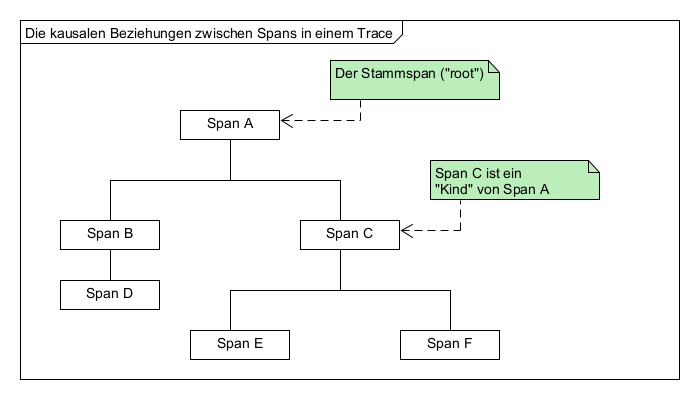
\includegraphics[width=\linewidth]{img/03_methoden/otel_causal-relationship.png}
	\captionof{figure}{Kausale Beziehung zwischen Spans. Eigene Darstellung.}
	\label{fig:otel-causal-relationship}
\end{minipage}%
\hspace{.06\textwidth}
\begin{minipage}{.47\textwidth}
	\centering
	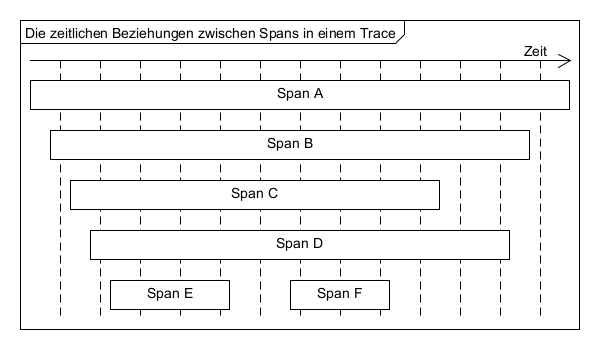
\includegraphics[width=\linewidth]{img/03_methoden/otel_temporal-relationship}
	\captionof{figure}{Zeitliche Beziehung zwischen Spans. Eigene Darstellung.}
	\label{fig:otel-temporal-relationship}
\end{minipage}

\subsection{Fehlerberichte}

\begin{wrapfigure}[15]{r}{0.4\textwidth}
\centering
\vspace{-\baselineskip}
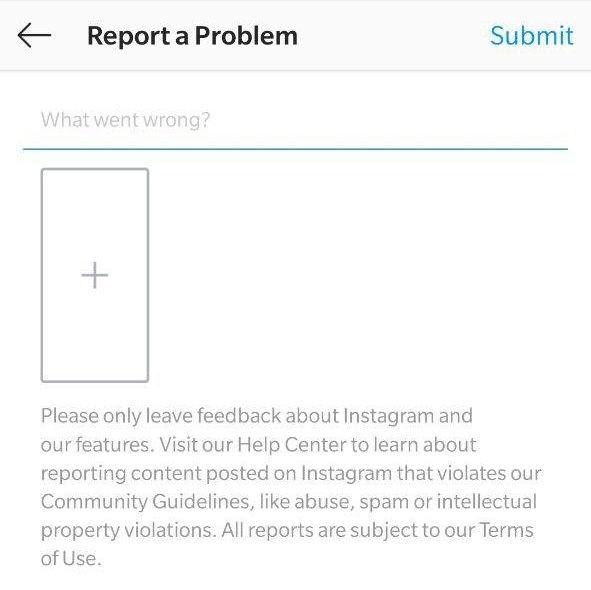
\includegraphics[width=\linewidth]{img/instagram-feedback/instagram-feedback.jpg}
\caption{Fehlerbericht in der Instagram App \cite{Instagram}}
\label{fig:instagram-bug-report}
\end{wrapfigure}

Fehlerberichte sind ein klassisches Mittel, um den Nutzer selber aktiv werden zu lassen und zu erfragen, welche Aktionen er durchgeführt hat und was schiefgelaufen ist (vgl \autoref{fig:instagram-bug-report}). Hiermit können Fehler, aber auch unverständliche Workflows, aufgedeckt werden. Weiterhin kann die Intention des Nutzers ermittelt werden, vorausgesetzt er gibt dies an.

Konträr zu den genannten  stehen jedoch die von Bettenburg \etal \cite{WhatMakesAGoodBugReport} gefunden Ergebnisse über die Effektivität von Fehlerberichten. Denn Nutzer meldeten Informationen und Details, die sich für die Entwickler als nicht allzu hilfreich herausstellten. Diese Diskrepanz kann u. A. dadurch erläutert werden, dass Nutzer im Regelfall kein technisches Verständnis vom System vorweisen.

\section{Praktiken}

In der Fachpraxis haben sich einige Technologien über die Jahre entwickelt und etabliert, welche die Nachvollziehbarkeit von Anwendungsverhalten und Nutzerinteraktion ermöglichen oder verbessern. Auf Basis der zuvor vorgestellten Methoden und teils neuen Ansätze haben sich in der Wirtschaft einige Praktiken entwickelt. Diese werden folgend näher beleuchtet.

\subsection{Observability}

In der Wirtschaft hat sich bei Werkzeugen, die auf eine verbesserte Nachvollziehbarkeit abzielen, der Begriff \enquote{Observability} etabliert,    um diese zu beschreiben. Es kann mit \enquote{Beobachtbarkeit} übersetzt werden, aber ließe sich auch freier mit Nachvollziehbarkeit gleichsetzen. Observability enstand aus dem klassischen Monitoring von Software, aber beinhaltet neben Monitoring noch einige weitere Disziplinen, wie Logging, Tracing und Metriken. Graf \cite{MichaelGrafBA} definiert Observability wie folgt:

%Observability hat allgemeiner als Ziel, dass Anwendungen und Systeme exakt betrachtet werden können, um den Verantwortlichen zu ermöglichen, dass  \cite{DistributedSystemsObservability}.

\begin{quotation}
Ziel ist es, Anwendungen und Systeme exakt zu beobachten, Informationen über technische Fehlfunktionen zu erhalten und schnell an die Verantwortlichen zu übermitteln. Logfiles, Informationen zur Ressourcennutzung und Anwendungs-Traces sollen den Administratoren und Entwicklern dabei helfen, die Fehlerursachen zu erkennen, die Probleme zu beheben und künftige Ausfälle nach Möglichkeit zu vermeiden \cite{DistributedSystemsObservability}.
\end{quotation}

\subsection{System Monitoring}

System Monitoring beschäftigt sich mit der Überwachung der notwendigen Systeme und Dienste in Bezug auf Hardware- und Softwareressourcen. Es handelt sich hierbei um ein projektunabhängiges Monitoring, welches sicherstellen soll, dass die Infrastruktur funktionstüchtig bleibt.

Ein Beispiel für System Monitoring wäre u. A., wenn man eine Menge an Systemen auf die Festplatten- und CPU-Auslastung hin kontrolliert und überwacht. Es können weitere Aspekte überwacht werden, aber im Regelfall hat die Überwachung selbst nichts mit einem eigentlichen Projekt zu tun, außer dass die Infrastruktur hierfür sichergestellt wird.

\subsection{Log Management}

Log Management umfasst die Erfassung, Speicherung, Verarbeitung und Analyse von Logdaten von Anwendungen. Neben den datenspezifischen Funktionen bieten solche Werkzeuge oftmals fundierte Suchfunktionen und Visualisierungsmöglichkeiten. Um die Daten aus einer Anwendung heraus zu exportieren, gibt es meist eine Vielzahl an Integrationen für Frameworks und Logbibliotheken.

Einer der wichtigsten Punkte beim Log Management, ist der Umgang mit großen Datenmengen und die gewünschten Operationen, die Nutzer damit durchführen möchten.

\subsection{Application Performance Monitoring (APM)}

Beim Application Performance Monitoring werden Messdaten innerhalb von Anwendungen gesammelt, um das Anwendungsverhalten nachvollziehbar zu gestalten \cite{StudyingTheEffectivenessOfAPMTools}. Auf Basis der Daten lassen sich u. A. Abweichungen von der Norm feststellen, von einzelnen Systemen oder vom aktuellen Gesamtsystem zu einem vorherigen Zeitpunkt.

Mithilfe von APM lassen sich allgemeine Aspekte von Software, wie die Ressourcennutzung, überprüfen aber auch spezielle Faktoren, wie die Ausführungszeit einer wichtigen Methoden, lassen sich so beleuchten. Die zu veranschaulichenden Aspekte werden zum Großteil über Metriken in numerische Werte abgebildet.

\subsection{Real User Monitoring (RUM)}

\nomenclature[Fachbegriff]{UI}{User-Interface}

Real User Monitoring beschäftigt sich mit dem Mitschneiden von allen Nutzerinteraktionen und Umgebungseigenschaften einer Webanwendung \cite{IdentifyingWebPerformanceDegradations}. Hiermit lässt sich nachvollziehen, wie ein Nutzer die Anwendung verwendet. RUM kann weiterhin dazu verwendet werden, um nachzuvollziehen, wie ein Zustand vom Nutzer erreicht worden ist. Aber es können auch ineffiziente Klickpfade hierdurch festgestellt werden und darauf basierend UX-Verbesserungen vorgenommen werden.

Weiterhin ist es beim RUM auch üblich Nutzerinteraktionen gruppierte zu analysieren, um verbreitete und unübliche Sitzungen zu identifizieren. Hiermit wird die Nutzerschaft und ihre Verhaltensweisen nachvollziehbarer gemacht.

\subsection{Synthetic Monitoring}

Beim Synthetic Monitoring werden Endnutzer simuliert, um Aspekte wie Funktionalität oder Verfügbarkeit zu verifizieren \cite{IdentifyingWebPerformanceDegradations}. Hierbei können Werkzeuge zur Browserautomatisierung eine echte Benutzung einer Webanwendung simulieren. Des Weiteren ist aber auch eine Nachstellung des Verhaltens der Webanwendung eine Option, indem z. B. Aufrufe zu Partnersystemen simuliert werden.

\subsection{Error/Crash Monitoring}

Das Error Monitoring konzentriert sich auf das Erfassen und Melden von Fehlern \cite{CrashbinCrashMonitoring}. Neben den eigentlichen Fehlern, werden meist alle verfügbaren Kontextinformationen mit erfasst. Darunter finden sich u. A. Daten aus den Gebieten RUM und Logging. Das Error Monitoring wird oftmals eng mit einem Issue-Management verbunden, da aufgetretene Fehler und deren Behebungen zu verfolgen sind \cite{CrashbinCrashMonitoring}.

\subsection{Session Replay}

Session Replay beschreibt das Vorgehen, eine Sitzung eines Nutzers nachzustellen, so als ob sie gerade passiert. Hierbei können einzelne Aspekte der Anwendung nachgestellt werden, bspw. der Kommunikationsablauf oder die DOM-Manipulationen. Desto mehr Aspekte nachgestellt werden, desto realitätsnaher ist die Nachstellung und entsprechend hilfreich ist sie beim Nachvollziehen.

Realitätsnahes Session Replay nimmt somit eine enorme Datenmenge für jede Nutzersitzung auf und benötigt besonders bei Browsern eine effiziente Kommunikation, um die UX nicht negativ zu beeinflussen.

\begin{wrapfigure}[10]{r}{0.40\textwidth}
\centering
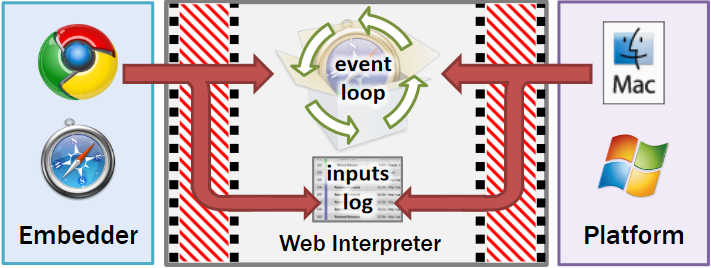
\includegraphics[width=\linewidth]{img/03_methoden/timelapse_figure5.png}
\caption{Mitschneiden von DOM-Events, Abb. aus \cite{TimelapsePaper}}
\label{fig:timelapse_figure5}
\end{wrapfigure}

Bereits 2013 entwickelten Burg \etal \cite{TimelapsePaper} mit \enquote{Timelapse} ein Framework, um Benutzersitzungen bei Webanwendungen aufzunehmen und wiederzugeben. Timelapse unterscheidet sich zu gängigen Session Replay-Ansätzen dahingehend, dass die Wiedergabe keine vereinfachte Nachstellung der Anwendung ist. Stattdessen wird die JavaScript-Eventloop abgekapselt und es werden die Aufrufe von und zu der Eventloop mitgeschnitten (vgl. \autoref{fig:timelapse_figure5}).

\begin{wrapfigure}[10]{r}{0.40\textwidth}
\centering
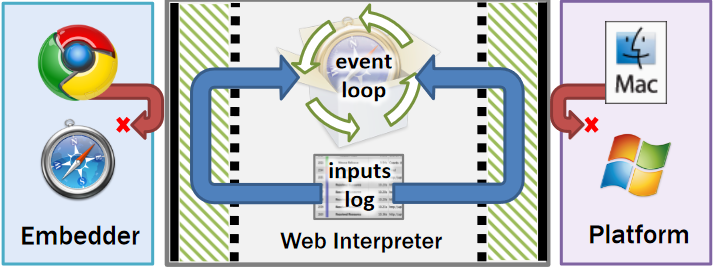
\includegraphics[width=\linewidth]{img/03_methoden/timelapse_figure6.png}
\caption{Abspielen von DOM-Events, Abb. aus \cite{TimelapsePaper}}
\label{fig:timelapse_figure6}
\end{wrapfigure}

Beim Abspielen werden die Aufrufe dann in derselben Reihenfolge an die Eventloop übergeben (vgl. \autoref{fig:timelapse_figure6}). Dies bedeutet es ist ein exaktes wiederholtes Ausführen in der selben Umgebung möglich, und dies ermöglicht eine detaillierte Nachvollziehbarkeit des Anwendungsverhaltens. Leider wird für diesen Ansatz eine gepatchte Version von WebKit benötigt, somit auch Zugriff auf das Endnutzersystem benötigt. Aus diesem Grund und weil es sehr mehr als 5 Jahren nicht mehr gepflegt wird\footnotemark{}, ist es ungeeignet für die hier angestrebte Lösung. Die vorgestellten Konzepte stellen jedoch nützliche Kernprinzipien für das Session Replay im Allgemeinen dar.

\footnotetext{Timelapse GitHub Repo \url{https://github.com/burg/replay-staging/}}

\section{Werkzeuge und Technologien}
\label{sec:werkzeuge-und-technologien}

%\textit{Basierend auf dem Grundwissen über die Methoden und Praktiken, soll nun der Stand der Technik erörtert werden. Hierbei sollen Werkzeuge und Technologien und ihre Ansätze hervorgehoben werden und mit Hilfe welcher Methoden sie welches Ziel erreichen.}
%
%\textit{Wie in der Zielsetzung definiert sollen hier zwei bis drei Technologien näher vorgestellt werden.}
%
%\textit{Weiterhin könnte beleuchtet werden, wie ähnliche Herausforderungen bei anderen „Fat-Client“-Lösungen (also nicht SPAs) angegangen werden, und kann man hier vielleicht etwas lernen oder übertragen (und wenn nicht, warum nicht)?}

%\subsection{Fachpraxis}

Bei der Recherche zu Werkzeugen und Technologien wurden einige Produkte aus Fachpraxis und Literatur näher betrachtet. Hierbei wurden die Technologien dahingehend evaluiert, ob sie für eine angestrebte Lösung in Frage kommen. Die Folgeabschnitte beschreiben die einzelnen Technologien, eine Auswahl erfolgt jedoch erst ist \autoref{sec:technologie-stack}. Weiterhin ist bei dieser Vorstellung keine bewertende Gegenüberstellung das Ziel gewesen.

Des Weiteren kam bei der Recherche wiederholt der Begriff \textbf{OpenTelemetry} auf, aufgrund dessen und aufgrund der Beziehung zu OpenTracing wird der Standard folgend kurz beschrieben.

\newpage

\subsection{OpenTelemetry}

\begin{wrapfigure}[19]{r}{0.35\textwidth}
\centering
\vspace{-3\baselineskip}
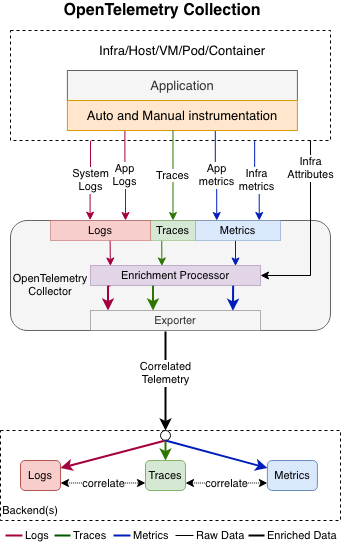
\includegraphics[width=\linewidth]{img/03_methoden/otel_unified-collection_2.png}
\caption{Schaubild einer Lösung auf Basis von OTel \cite{OpenTelemetryUnifiedCollection}}
\label{fig:otel-unified-collection}
\end{wrapfigure}

OpenTelemetry (OTel) \cite{OpenTelemetry} ist ein sich derzeit entwickelnder herstellerunabhängiger Standard, um Tracing-, Metrik- und Logdaten\footnotemark{} zu erfassen, zu verarbeiten, zu analysieren und zu visualisieren. OTel fasst die beiden Standards OpenTracing und OpenCensus \cite{OpenCensus} zusammen und hat sich als Ziel gesetzt diese zu erweitern \cite{UseNixDistributiveTracing}. Hinter dem Standard stehen u. A. die Cloud Native Computing Foundation (CNCF), Google, Microsoft, und führende Hersteller von Tracing- und Monitoring-Lösungen. Ein erster Release ist für Ende 2020/Anfang 2021 geplant. Ziel ist es, dass Entwickler Tools und Werkzeuge benutzen können, ohne erneut hochspezifische Anbindungen schreiben und konfigurieren zu müssen. Stattdessen definiert der Standardkomponenten, die spezielle Aufgabengebiete haben und mit einer allgemeinen API anzusprechen sind. Die technische Infrastruktur einer auf OTel basierenden Lösung ist in \autoref{fig:otel-unified-collection} zu sehen. Im groben definiert OTel folgende Komponenten: API, SDK, Exporter, Collector und Backend (vgl. \autoref{fig:otel-components}).

In der Bachelorarbeit von Graf \enquote{Bedeutung von Telemetrie für den Software-Development-Life-Cycle} \cite{MichaelGrafBA} beschäftigt sich Graf intensiv mit dem Einfluss und dem Nutzen von Telemetrie in modernen Softwareprojekten. Speziell beschreibt er den OTel Standard und seine Bedeutung im aktuellen Gebiet der Telemetrie. Er bewertet die Entwicklung des Standards positiv, besonders auf Basis der Aspekte Interoperabilität, Plattformunabhängigkeit und Erweiterbarkeit. Jedoch mahnt er zudem, dass das Projekt noch jung ist und keine Prognosen über den Erfolg gemacht werden können. Grafs Arbeit sichert somit zu, dass OpenTelemetry ein, nicht zu vernachlässigender, Standard im Gebiet der Observability darstellt.

\nomenclature[Fachbegriff]{OTel}{OpenTelemetry}
\nomenclature[Fachbegriff]{CNCF}{Cloud Native Computing Foundation}
\footnotetext{Logging ist noch nicht gut im OTel Standard definiert/aufgenommen \cite{OpenTelemetryLoggingSpecification}}

\begin{figure}[H]
	\centering
	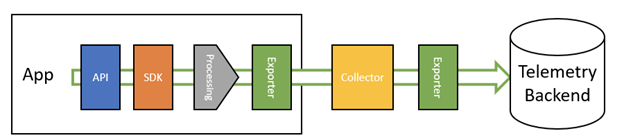
\includegraphics[width=0.55\linewidth]{img/03_methoden/dynatrace_otel-components.png}
	\caption{OTel Komponenten \cite{DynatraceOTelComponents}}
	\label{fig:otel-components}
\end{figure}

\subsection{Weiteres}
\label{sec:weitere-werkzeuge}

Bei der Recherche und Evaluierung wurden nicht alle auf dem Markt verfügbaren Werkzeuge und Technologien tiefergehend betrachtet. Deshalb werden weitere Funde, die nicht betrachtet wurden, hier kurz notiert:

\begin{itemize}
	\item APM \& RUM: AppDynamics, DataDog
	\item Error Monitoring: Airbrake, Instabug, Rollbar, Bugsnag, TrackJS
	\item Tracing oder Observability: Google Cloud Trace, Zipkin, Logz.io, Lightstep
\end{itemize}

Auch diese Auflistung stellt nicht die komplette Bandbreite an Werkzeugen und Technologien dar und die vorhergehende Betrachtung ist nicht als Empfehlung zu verstehen.

\subsection{New Relic}

New Relic \cite{NewRelic} ist eine Software-as-a-Service (SaaS) der gleichnamigen Firma, welcher Betreiber von Softwareprojekten dabei unterstützt das Verhalten ihrer Anwendungen zu überwachen. Der Dienst konzentriert sich auf System Monitoring, APM und RUM und erfasst die notwendigen Daten mit proprietären Lösungen. Neben den Kernfunktionalitäten unterstützt New Relic auch Log Management, Synthetic Monitoring, Tracing und Error Monitoring.

\nomenclature[Fachbegriff]{SaaS}{Software-as-a-Service}

New Relic steht sowohl als kostenlose sowie als kommerzielle Lösung zur Verfügung. Da die kostenlose Version aber benötigte Features abdeckt, wurde diese im Rahmen der Arbeit eingesetzt. Der New Relic Agent, welcher die Daten beim Client sammelt, wird über ein Skript eingebunden und sendet in regelmäßigen Abständen Daten an New Relic. Über die Oberfläche von New Relic können dann allgemeine Charakteristika der Clients betrachtet werden, wie Ladezeiten, Browserhersteller, Ajax-Antwortzeiten. Spezielle Eigenschaften eines einzelnen Nutzers sind jedoch nicht möglich auszulesen. Im Fehlerfall stehen jedoch mehr Informationen, wie Stacktrace, genaue Browserversion, Uhrzeit zur Verfügung und in der Oberfläche dargestellt.

Mithilfe dieser Informationen erhält ein Entwickler oder Betreiber einen guten Rahmen, um die Umgebung als solches zu verstehen und den eigentlichen Fehler einzusehen. Jedoch geben diese Informationen nicht darüber Aufschluss, wie es zu dem Fehler kam, also welche Ereignisse direkt dem Fehler vorgelagert waren - es sind unter anderem keine Logdaten einzusehen.

New Relic bietet darüber hinaus eine Unterstützung von OTel-Daten  \cite{NewRelicAnnoundOTelBetaSupport}, welches jedoch nicht mit evaluiert werden konnte, da es in der kostenlosen Version nicht enthalten war. Auf der offiziellen Seite von OTel werden jedoch  öffentliche Exporter für New Relic angeboten \cite{OpenTelemetryRegistry}.

\subsection{Dynatrace}

Dynatrace \cite{Dynatrace} ist eine SaaS-Lösung des gleichnamigen Unternehmens und ähnelt im Funktionsumfang stark New Relic. Es werden wie bei New Relic die Kernfunktionalitäten APM und RUM, sowie die Disziplinen Log Management, Synthetic Monitoring, Tracing und Error Monitoring.

Dynatrace bietet neben dem kostenpflichtigen Dienst eine 14-tägige Testversion dessen, welche im Rahmen dieser Arbeit verwendet wurde. Die Datenerhebung erfolgt über den Dynatrace OneAgent, welcher genauso wie New Relics Agent kontinuierlich Daten sendet. In der Oberfläche von Dynatrace sind ähnliche Datenkategorien zu finden, wie bei New Relic, wobei Dynatrace diese visuell ansprechender darstellt. Dynatrace bietet zudem auch die Funktionalität des Error Monitoring, aber leidet unter demselben Problem wie New Relic: zu wenig Kontextinformationen.

Dynatrace ist zudem dem OpenTelemetry Team beigetreten und hat angegeben, an der Weiterentwicklung mitzuhelfen \cite{DynatraceJoinOTelProject}. Eine Integration des Dienstes Dynatrace ins Ökosystem von OTel gibt es jedoch noch nicht.

\subsection{Sentry}

Sentry \cite{Sentry} ist ein SaaS-Produkt der Functional Software Inc., welcher sich auf das Error Monitoring spezialisiert. Die Kernfunktionalitäten beschränken sich auf das Error Monitoring, auch wenn von anderen Praktiken einige Aspekte präsent sind, stellen diese keine eigens abgeschlossene Funktionalität dar.

Neben einer kommerziellen Version, bietet Sentry auch eine unbegrenzte kostenlose Version bereit, welche im Rahmen dieser Arbeit evaluiert wurde. Um von Webanwendungen Fehler zu erfassen und an Sentry zu melden, bietet Sentry bei NPM quelloffene Pakete an \cite{SentryJSGithub}. Dabei werden Pakete für folgende Frameworks bereitgestellt: JavaScript, Angular, AngularJS, Backbone, Ember, Gatsby, React und Vue.

Anders als bei den beiden vorherigen Tools wird zu Sentry nur kommuniziert, wenn ein Fehler auftritt. Hierbei werden dafür aber umso mehr Daten erhoben: Detaillierte Klickpfade des Nutzers, Logmeldungen der Browserkonsole sowie die Informationen, die auch die anderen Tools bereitstellen.

In der Oberfläche von Sentry werden die gemeldeten Fehler in sogenannten \enquote{Issues} zusammengefasst. Diese entsprechen Fehlertickets und die Oberfläche erlaubt eine Zuweisung dieser Tickets sowie ein detailliertes Nachhalten der Fehlerbehebung.

Die angeboten Fehlerinformationen von Sentry sind zahlreich und helfen beim Nachvollziehen besser als die vorher beleuchteten Werkzeuge, jedoch mangelt es an einer ganzheitlichen Nachvollziehbarkeit auch in nicht Problemszenarien.

Der Quellcode von Sentry wurde veröffentlicht und weiterhin wird bei Sentry auch eine OnPremise-Lösung, basierend auf Docker, angeboten \cite{SentrySelfHosted}.

\subsection{LogRocket}

LogRocket \cite{LogRocket} ist ein SaaS-Produkt des gleichnamigen Unternehmens und konzentriert sich auf detailliertes Session Replay von JavaScript-basierten Clientanwendungen, um Probleme identifizieren, nachvollziehen und lösen zu können.

LogRocket bietet eine kostenlose Testversion des SaaS-Produktes an
Für die Evaluierung wurde die kostenlose Testversion von LogRocket verwendet. Zur Datenerhebung wurde das Paket \texttt{logrocket} von NPM hinzugezogen und nach der Initialisierung sammelt es eigenständig die notwendigen Daten. Mithilfe der gesammelten Daten wird die gesamte Sitzung des Nutzers nachgestellt. Hierbei ist die Anwendung, die Nutzerinteraktionen, die Netzwerkaufrufe sowie das DOM zu sehen. Die Reproduktion wird videoähnlich aufbereitet und erlaubt ein präzises Nachvollziehen der zeitlichen Reihenfolge und Bedeutung (vgl. \autoref{fig:logrocket-Session Replay-example}).

Neben dem JavaScript SDK bietet LogRocket quelloffenene Plugins für folgende Bibliotheken: Redux, React, MobX, Vuex, ngrx, React Native. LogRocket ist zudem als OnPremise-Lösung verfügbar. Zusätzlich bietet LogRocket auch Integration für andere Tools, wie z. B. Sentry. Bei der Integration zu Sentry wird bei einem gemeldeten Fehler direkt auf das \enquote{Video} in LogRocket verlinkt, sodass der Fehler genau betrachtet werden kann.

\begin{figure}[H]
	\centering
	\includegraphics[width=\linewidth]{img/03_methoden/logrocket_Session Replay-example.png}
	\caption{Beispiel eines Session Replays bei LogRocket}
	\label{fig:logrocket-Session Replay-example}
\end{figure}

\subsection{Splunk}

Splunk \cite{Splunk} ist ein Softwareprodukt und eine SaaS-Lösung des gleichnamigen Unternehmens. Splunk fungiert als eine universelle Datensenke, z. B. für Metriken und Logdaten. Es bietet Funktionen diese Daten zu durchsuchen, überwachen, analysieren und visualisieren. Weiterhin wird Splunk klassisch für Log Management eingesetzt, kann aber auch Aspekte von APM, RUM und Error Monitoring erfüllen.

Splunk bietet neben kostenpflichtigen Versionen der SaaS- und OnPremise-Lösung jeweils kostenlose Varianten an, welche in dieser Arbeit zur Evaluierung herangezogen wurden. Splunk selber bietet keine JavaScript-Pakete an, um Daten von einer Webanwendung an Splunk zu senden. Jedoch ist eine HTTP-Schnittstelle vorhanden mit der eigene Datensätze in Splunk gespeichert werden können.

Über diese HTTP-Schnittstelle wurden aus der Webanwendung einerseits Loginformationen gesendet, aber auch Fehlerdaten, wie man sie z. B. bei Sentry finden konnte. Die Daten ließen sich effizient in Splunk manuell durchsuchen, filtern, und visualisieren. Durch den Fakt, dass Splunk als dieselbe Datensenke für Fehler- und Loginformationen agierte, erlaubte die Kombination aus diesen beiden Datenkategorien. Speziell heißt dies, dass man bei Fehlerfällen direkt zu den Loginformationen zur selben Sitzung wechseln konnte.

Jedoch ist das Error-Monitoring nicht vergleichbar gut wie das von Sentry, da die Funktionalität des Issue-Managements nicht vorhanden ist. Weiterhin wurde evaluiert, ob auch Tracingdaten in Splunk aufgenommen werden können, aber hierbei besitzt Splunk keine gängigen Visualisierungen, wie ein Trace-Gantt-Diagramme.

\subsection{Honeycomb}

Honeycomb \cite{Honeycomb} ist eine SaaS-Lösung der Hound Technology Inc. und verspricht die Speicherung vieler (Tracing-)Daten und darauf basierend effiziente Abfragen zu ermöglichen. Es ist hauptsächlich als Tracingdienst anzusehen, womit jedoch auch Aspekte des APM, RUM und Error Monitoring mit abgebildet werden können.

Honeycomb wurde mit der kostenlosen Version evaluiert. Honeycomb bietet sog. \enquote{Beelines} an, welche Werkzeuge zur automatischen Datenerfassung sind. Diese Beelines sind für Node.js, Go, Python, Java, Ruby und Rails verfügbar. Da keine Beelines für JavaScript in Browsern verfügbar ist, wurden die Daten mit OTel-Komponenten erhoben und ein eigener Exporter für Honeycomb entwickelt.

Honeycomb konzentriert sich auf die Datenkategorien Tracing und Metriken, ähnlich wie der Standard OpenTelemetry. Dabei bietet Honeycomb in der Oberfläche Möglichkeiten selber Graphen auf Basis der Daten zu erstellen. Somit ist dies keine ausgefertigte Lösung, wie es teils bei New Relic und Dynatrace zu finden ist und kann somit auf die Anforderungen des Projektes besser angepasst werden. Jedoch ist dieser Ansatz mit einem höheren Aufwand und einer notwendigen Expertise verbunden.

\subsection{Jaeger}

Jaeger wurde 2017 als ein OpenSource-Projekt der CNCF gestartet \cite{Jaeger}. Es ist ein System für verteiltes Tracing und bietet Funktionalitäten zur Datensammlung, -verarbeitung, -speicherung bis hin zur Visualisierung. Jaeger unterstützt und implementiert den Standard OpenTracing, unterstützt aber auch Datenformate anderer Hersteller (wie z. B. Zipkin). Eine Unterstützung des OpenTelemetry Standards ist derzeit im Gange. Weiterhin kann Jaeger dazu benutzt werden, Metriken nach Prometheus \cite{Prometheus} zu exportieren, einem weiteren CNCF Projekt zur Speicherung und Visualisierung von Daten.

\begin{wrapfigure}[13]{r}{0.45\textwidth}
\centering
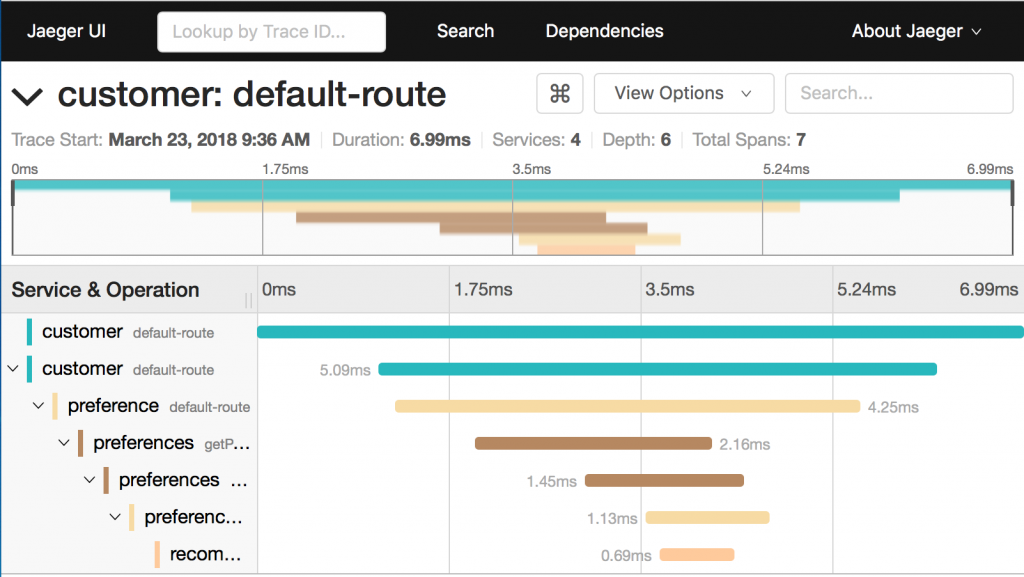
\includegraphics[width=\linewidth]{img/03_methoden/redhat_jaeger-ui_trace-detail-view.png}
\caption{Trace-Detailansicht. Quelle: Don Schenck \cite{JaegerIstioTracing}}
% von https://developers.redhat.com/blog/2018/04/03/istio-tracing-monitoring/
\label{fig:jaeger-ui_trace-detail-view}
\end{wrapfigure}

Jaeger spezialisiert sich auf Tracing und bietet hierfür eine skalierbare Infrastruktur zur Speicherung und Analyse der Daten. Die Traces werden als angereicherte Trace-Gantt-Diagramme dargestellt, wie in \autoref{fig:jaeger-ui_trace-detail-view} zu sehen ist. Hierbei sind sowohl hierarchische als auch zeitliche Beziehungen visualisiert. Wie bei OpenTracing und OpenTelemetry besteht ein Trace aus mehreren Spans, welche meist eine Methode umschließen. Zu den einzelnen Spans lassen sich weitere Informationen anzeigen, wenn vorhanden, wie bspw. Logmeldungen oder Kontextinformationen.

\begin{wrapfigure}[10]{r}{0.45\textwidth}
\centering
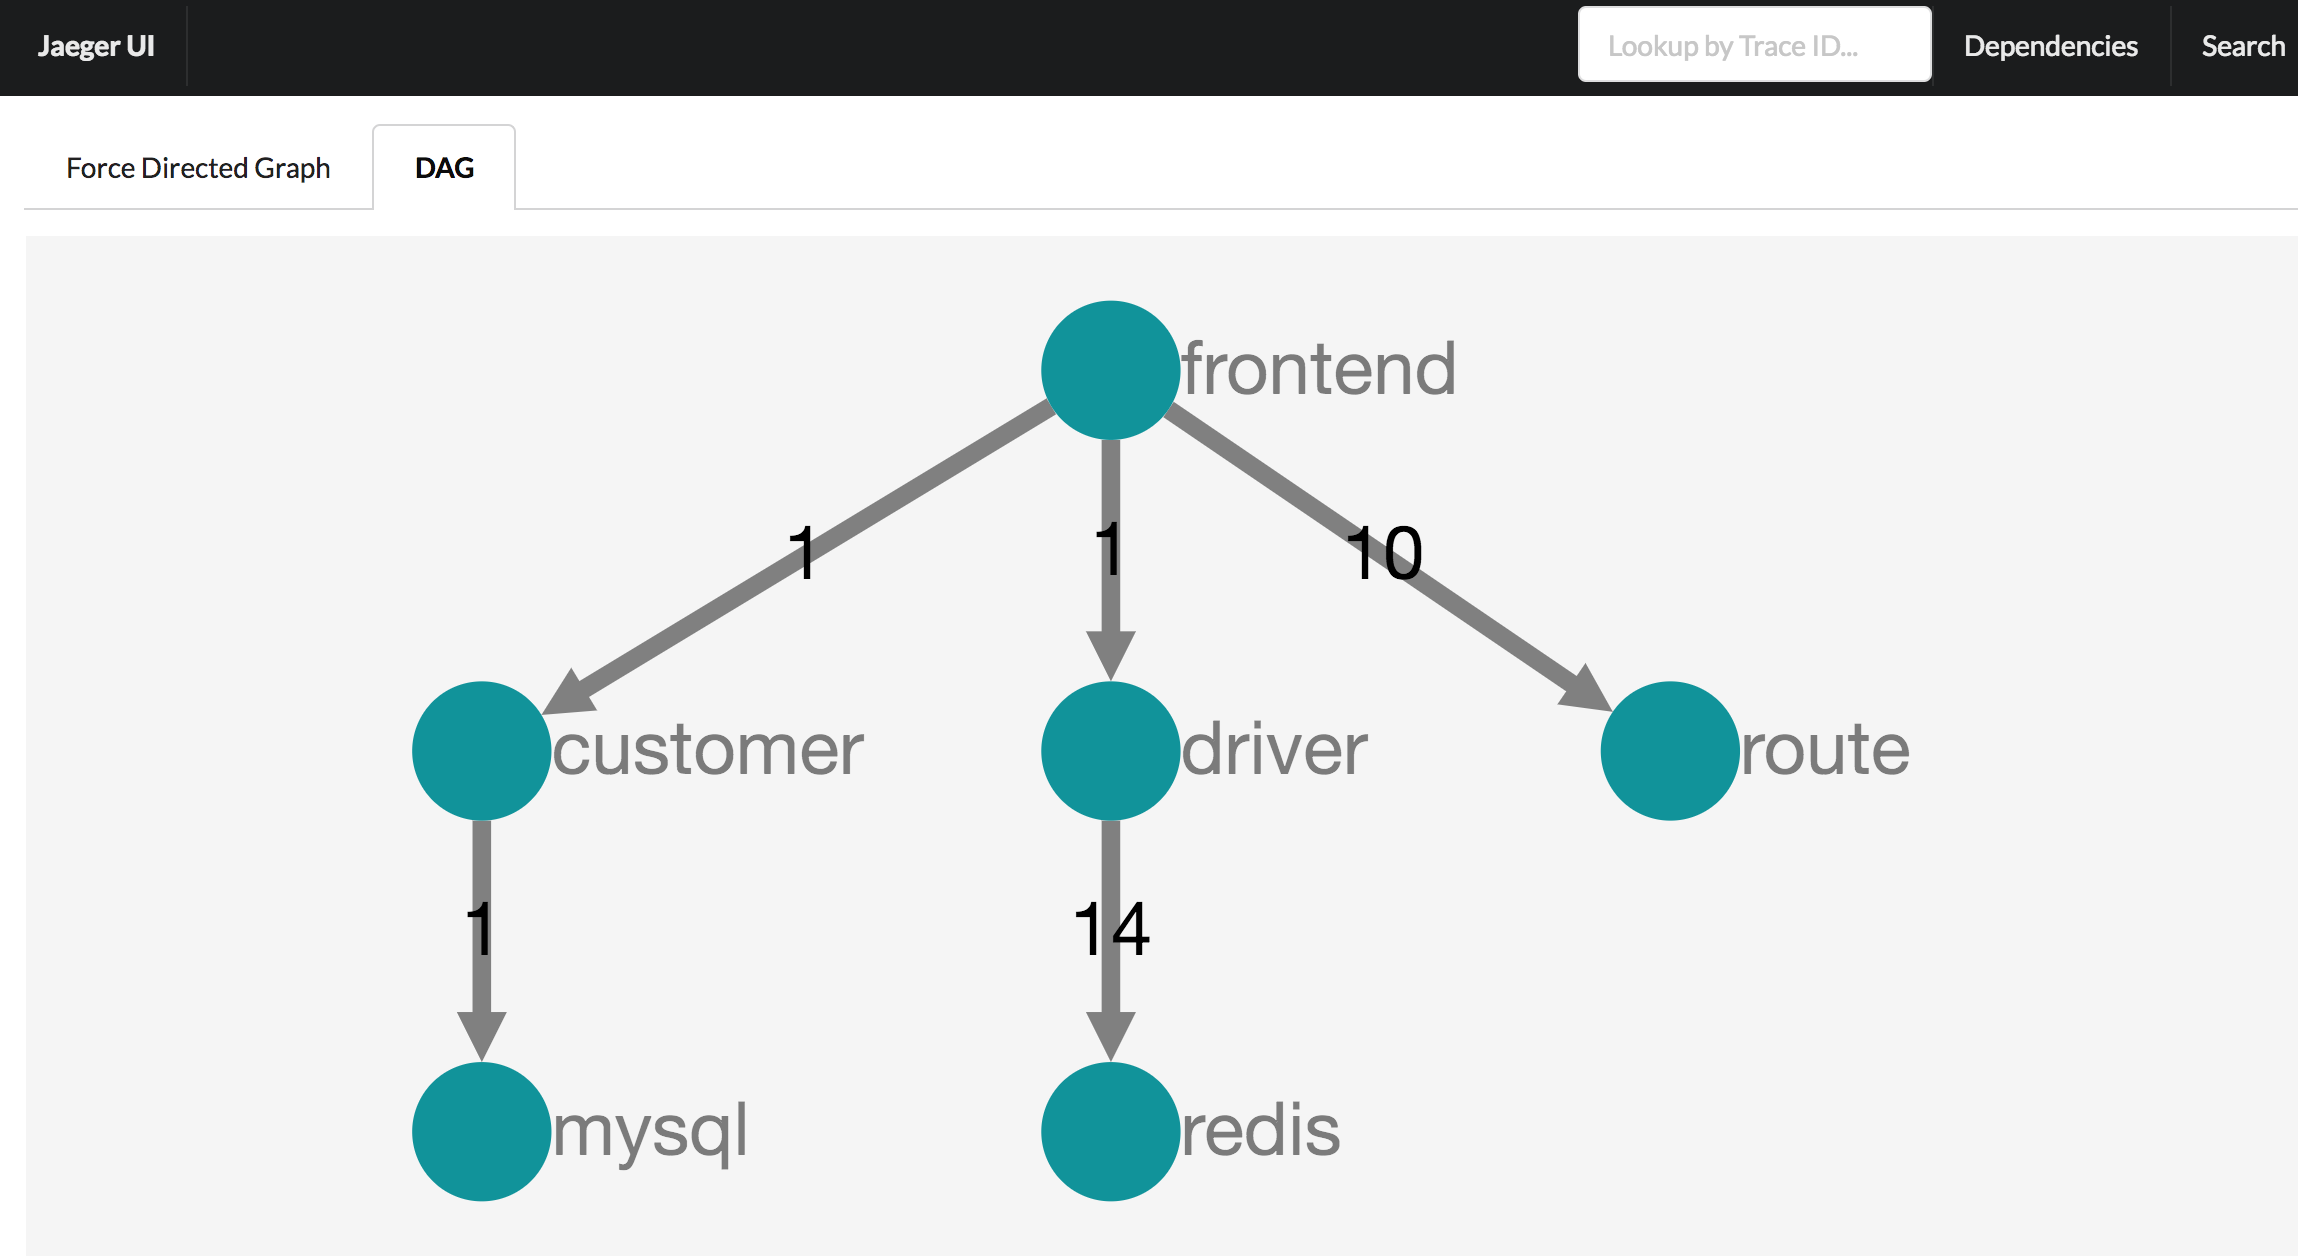
\includegraphics[width=\linewidth]{img/03_methoden/medium_jaeger-ui_dependency-graph.png}
\caption{Dienst-Abhängigkeits-Graph. Quelle: Yuri Shkuro \cite{JaegerTakeOpenTracingForARide}}
% von https://medium.com/opentracing/take-opentracing-for-a-hotrod-ride-f6e3141f7941
\label{fig:jaeger-ui_dependency-graph}
\end{wrapfigure}

Anhand der Traces generiert Jaeger zudem automatisch eine Architektur, indem die Beziehungen zwischen Diensten zu sehen ist. In \autoref{fig:jaeger-ui_dependency-graph} kann so eine Darstellung betrachtet werden.

\subsection{TraVista}

Passend zu Jaeger konnte in der Literatur ein Werkzeug identifiziert worden, welches auf bestehende Visualisierungen mittels Trace-Gantt-Diagrammen aufsetzt und diese erweitert. Anand \etal \cite{TraVistaPaper} argumentieren in ihrem Bericht, dass Visualisierungen rund ums Tracing zu strikt die unterschiedlichen Daten einer Anwendung trennen, statt diese zu kombinieren und strukturiert zu veranschaulichen. Mit TraVista haben die Autoren Visualisierungen erstellt, die genau diese Verknüpfung der unterschiedlichen Datentypen versuchen.

\begin{wrapfigure}[8]{r}{0.3\textwidth}
\centering
\vspace{-1.5\baselineskip}
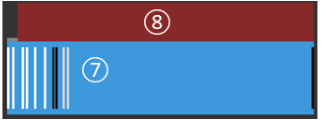
\includegraphics[width=\linewidth]{img/03_methoden/travista_extended-gantt_zoomed-in.png}
\caption{Zoom von \autoref{fig:travista_extended-gantt}, Abbildung aus \cite{TraVistaPaper}}
\label{fig:travista_extended-gantt_zoomed-in}
\end{wrapfigure}

In der Oberfläche von TraVista werden Metriken, Events sowie Tracedaten simultan dargestellt, um dem Nutzer ein komplementäres Bild des eigentlichen Traceverlaufs zu präsentieren. Diese Visualisierung kann in \autoref{fig:travista_extended-gantt} betrachtet werden, und ein Zoom ist bei \autoref{fig:travista_extended-gantt_zoomed-in} zu finden. Das Trace-Gantt-Diagramm wurde u. A. bei \circled{2} um einige Metriken erweitert, wobei der aktuelle Trace hervorgehoben im Vergleich zu anderen Traces dargestellt wird. Weiterhin lassen sich im Zoom bei \circled{7} aufgetretene Events als Balken betrachten, wobei selten aufgetretene Events schwarz hervorgehoben werden.

Leider ist TraVista keine ausgereifte Software und wird seit einigen Monaten nicht mehr weiterentwickelt\footnotemark{}. Aufgrund dessen wird es in dieser Arbeit nicht verwendet, dennoch zeigt sich durch den Bericht, dass bestehende und etablierte Produkte wie Jaeger und Zipkin ein Verbesserungspotenzial aufweisen.

\footnotetext{TraVista auf GitHub: \url{https://github.com/vaastav/TraViz}}

\begin{figure}[H]
	\centering
	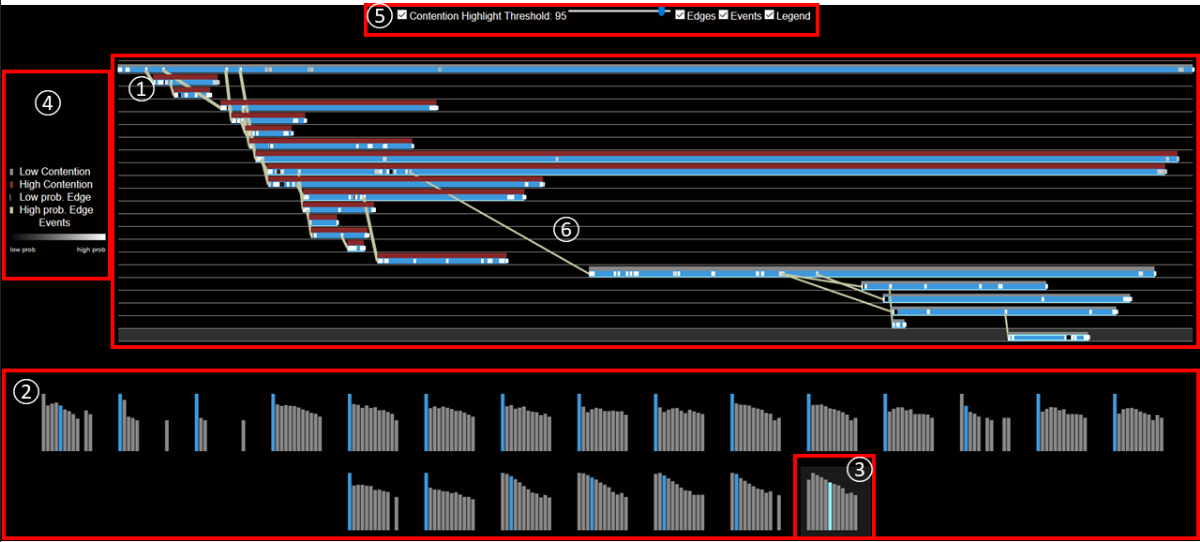
\includegraphics[width=0.815\linewidth]{img/03_methoden/travista_extended-gantt.png}
	\caption{TraVistas Gantt-Diagramm, Abbildung aus \cite{TraVistaPaper}}
	\label{fig:travista_extended-gantt}
\end{figure}

\subsection{FAME}

2018 arbeiteten Oriol \etal \cite{FamePaper} mit der Firma SEnerCon GmbH zusammen, um ein Framework zu Erstellen, welches Daten aus Nutzerfeedback und Monitoring kombiniert. SEnerCon wurde hinzugezogen, um das Framework zu evaluieren, die Entwicklung des Frameworks fand durch die Forscher selbst statt. Das Framework wurde FAME\footnotemark{} genannt und steht für \enquote{Feedback Acquisition and Monitoring Enabler}.

\footnotetext{FAME auf GitHub: \url{https://github.com/supersede-project/monitor_feedback}}

In dem Bericht wurde erforscht, ob die kombinierten Daten aus Nutzerfeedback und Monitoring dabei helfen können, um neue Anforderungen zu ergründen. Auf Basis dieser Forschungsfrage wurde das Framework erstellt und es konnte am Ende ein Mehrwert für die SEnerCon GmbH identifiziert werden.

\subsection{The Kaiju Project}

Scrocca \etal \cite{TheKaijuProjectPaper} identifizierten 2020 eine Lücke im Gebiet der Observability, nämlich fehlt ein Werkzeug, welches die unterschiedlichen Datentypen Logs, Traces und Metriken kombiniert sammeln und aufbereiten kann und dies in quasi-Echtzeit. Aus diesem Mangel ergab sich die Forschungsfrage, ob eine Kombination dieser Datenkategorien einen Mehrwehrt für die Nachvollziehbarkeit bedeuten kann.

Um die Forschungsfrage zu beantworten wurde ein Prototyp konzipiert, welcher genau diese Datenkategorien aggregiert und diese zu High-Level-Events zusammenfasst. Bei der Evaluierung mit der IT Dienstleistungsfirma SighUp konnte festgestellt werden, dass die resultierenden High-Level-Events hilfreiche Informationen zur Problemfindung beinhalten.

Das Projekt Kaiju hat bisher nicht die Phase des Prototypen verlassen und wird seit einigen Monaten auch nicht weiterentwickelt\footnotemark{}. Jedoch ist die Erkenntnis, dass die Kombination von Daten unterschiedlicher Quellen und Kategorien einen Mehrwert bietet, eine wegbereitende für diese Arbeit und die angestrebte Lösung. Somit wird in der hier angestrebten Lösung auch versucht unterschiedliche Kategorien miteinander zu verknüpfen, um Synergieeffekte für die Betreiber und Entwickler zu erzeugen. Folgend wird mit der Konzeption und Erstellung des Proof-of-Conceptes fortgesetzt.

\footnotetext{Kaiju auf GitHub: \url{https://github.com/marioscrock/Kaiju}}

%\subsection{Fazit zur Literatur}
%
%Wie in den verschiedenen beleuchteten Berichten und Arbeiten zu lesen ist, von denen drei in \textit{2020} veröffentlicht wurden, ist das Forschungsfeld der Nachvollziehbarkeit bzw. der Observability bisher nur spärlich untersucht worden. Eigene Recherchen ergaben das gleiche Ergebnis, das Feld enthält wenige konkrete Veröffentlichungen. Speziell zur Nachvollziehbarkeit im Bereich der Frontend-Entwicklung konnte keine Arbeit gefunden werden.
%
%Es konnte jedoch ein Konsens identifiziert werden, dass dieses Forschungsfeld einen wichtigen Mehrwert darstellt, speziell bei komplexen Microservice-Architekturen. Weiterhin lässt sich ein steigender Trend in konkreten Lösungsansätzen im Forschungsfeld identifizieren, wie u. A. die in dieser Arbeit näher betrachteten Veröffentlichungen. Diese Entwicklung geht einher mit den Standardisierungsbemühungen aus der Wirtschaft rund um OpenTelemetry.
%
%Nun da die theoretische Seite der Nachvollziehbarkeit beleuchtet wurde, wird sich nun mit der Erstellung eines eigenen Konzeptes und der Anwendung dessen beschäftigt.